%%%%%%%%%%%%%%%%%%%%%%%%%%%%%%%%%%%%%%%%%%%%%%
%                insertmeeting
% 1) Title (something creative & funny?)
% 2) Date (MM/DD/YYYY)
% 3) Location (ex. Hagerty High School)
% 4) People/Committees Present 
% 5) Picture 
% 6) Start Time & Stop Time (ex. 12:30AM to 4:30PM)
%%%%%%%%%%%%%%%%%%%%%%%%%%%%%%%%%%%%%%%%%%%%%%
\insertmeeting 
	{Pi Day!} 
	{03/14/22} 
	{Hagerty High School}
	{James, Jensen, Nathan, Ritam}
	{Images/RobotPics/robot.jpg}
	{2:30 - 8:30}
	
\hhscommittee{Hardware}
\noindent\hfil\rule{\textwidth}{.4pt}\hfil
\subsubsection*{Goals}
\begin{itemize}
    \item Attempt to use a UCF CNC Router constructed by past senior students. 

\end{itemize} 

\noindent\hfil\rule{\textwidth}{.4pt}\hfil

\subsubsection*{Accomplishments}
Today, our UCF mentor suggested we look at the Innovation Lab CNC router over spring break. The machine was built by UCF students as a senior design project two years prior. We wanted to use the CNC router to cut a sheet of carbon fiber for our intake plates. The first step was using a maker space software to convert our CAD drawings into the format for the CNC router. We spent a few hours playing with the various drawing tools for to align the CAD outline correctly. One of the first problems that we encountered was the drill bits. The software did not have preset profiles for our metric-labeled drill bit. We then had to measure the diameter and flutes for the profile. However, we later realized the drill bit was exactly the same size as an imperial 1/8th drill bit, so we could just use that profile instead. Very cool. The next problem was actually using the machine. The screen and keyboard were both small, making them a little hard to read. In addition, the designers added two USB ports when three would be needed for actual operation (Mouse, keyboard, and a USB drive with the file to cut). After slowly putting the file on the machine using a keyboard and the USB, we were finally ready to cut. The process involved setting the drill home by manually moving the bit and zeroing out the positions. We performed a "dry run" to ensure that the drill was moving in the correct path. The dry run was successful, so we ran it with the drill bit down. Even though the drill went through the carbon fiber, it did not go all the way through in some places. The error might have been caused by a drill bit. However, this was a good test run overall, since we were able to prove that the CNC router works. 



\begin{figure}[htp]
\centering
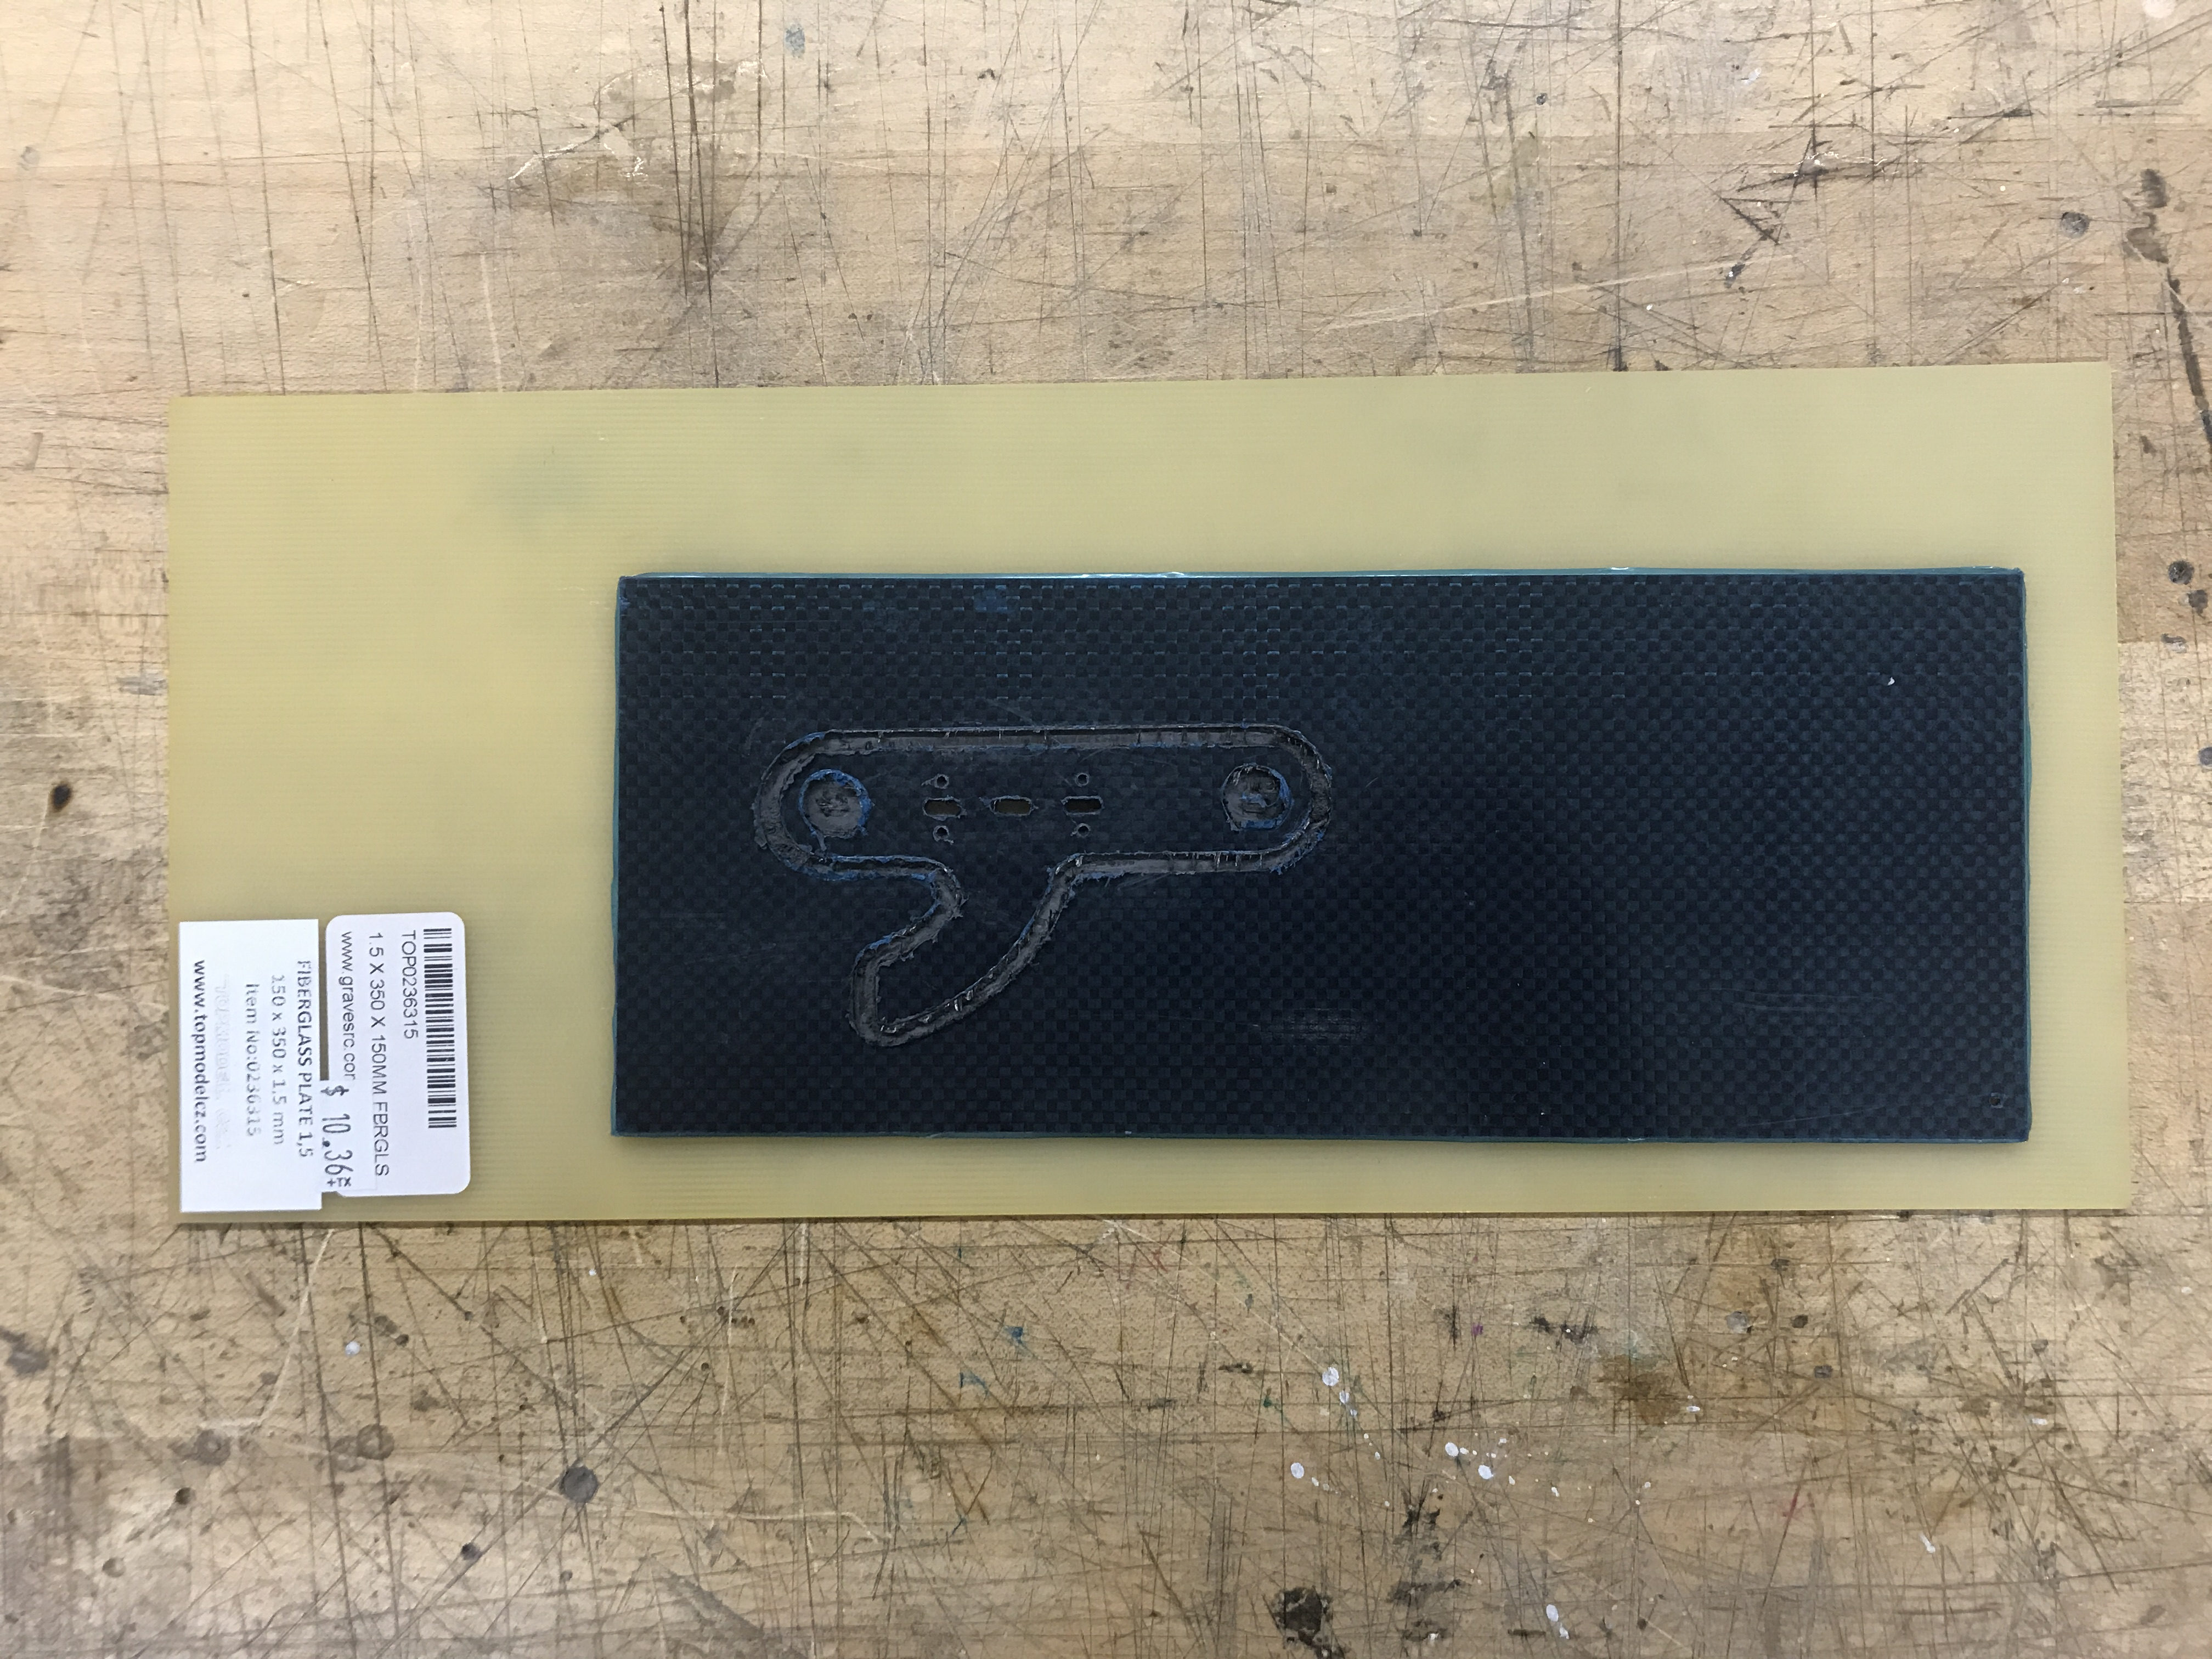
\includegraphics[width=0.95\textwidth, angle=0]{Meetings/March/03-14-22/03-14-22 1.JPG}
\caption{The final cut out of the carbon fiber plate. The drill bit didn't go all the way through.}
\label{fig:031022_1}
\end{figure}

\begin{figure}[htp]
\centering
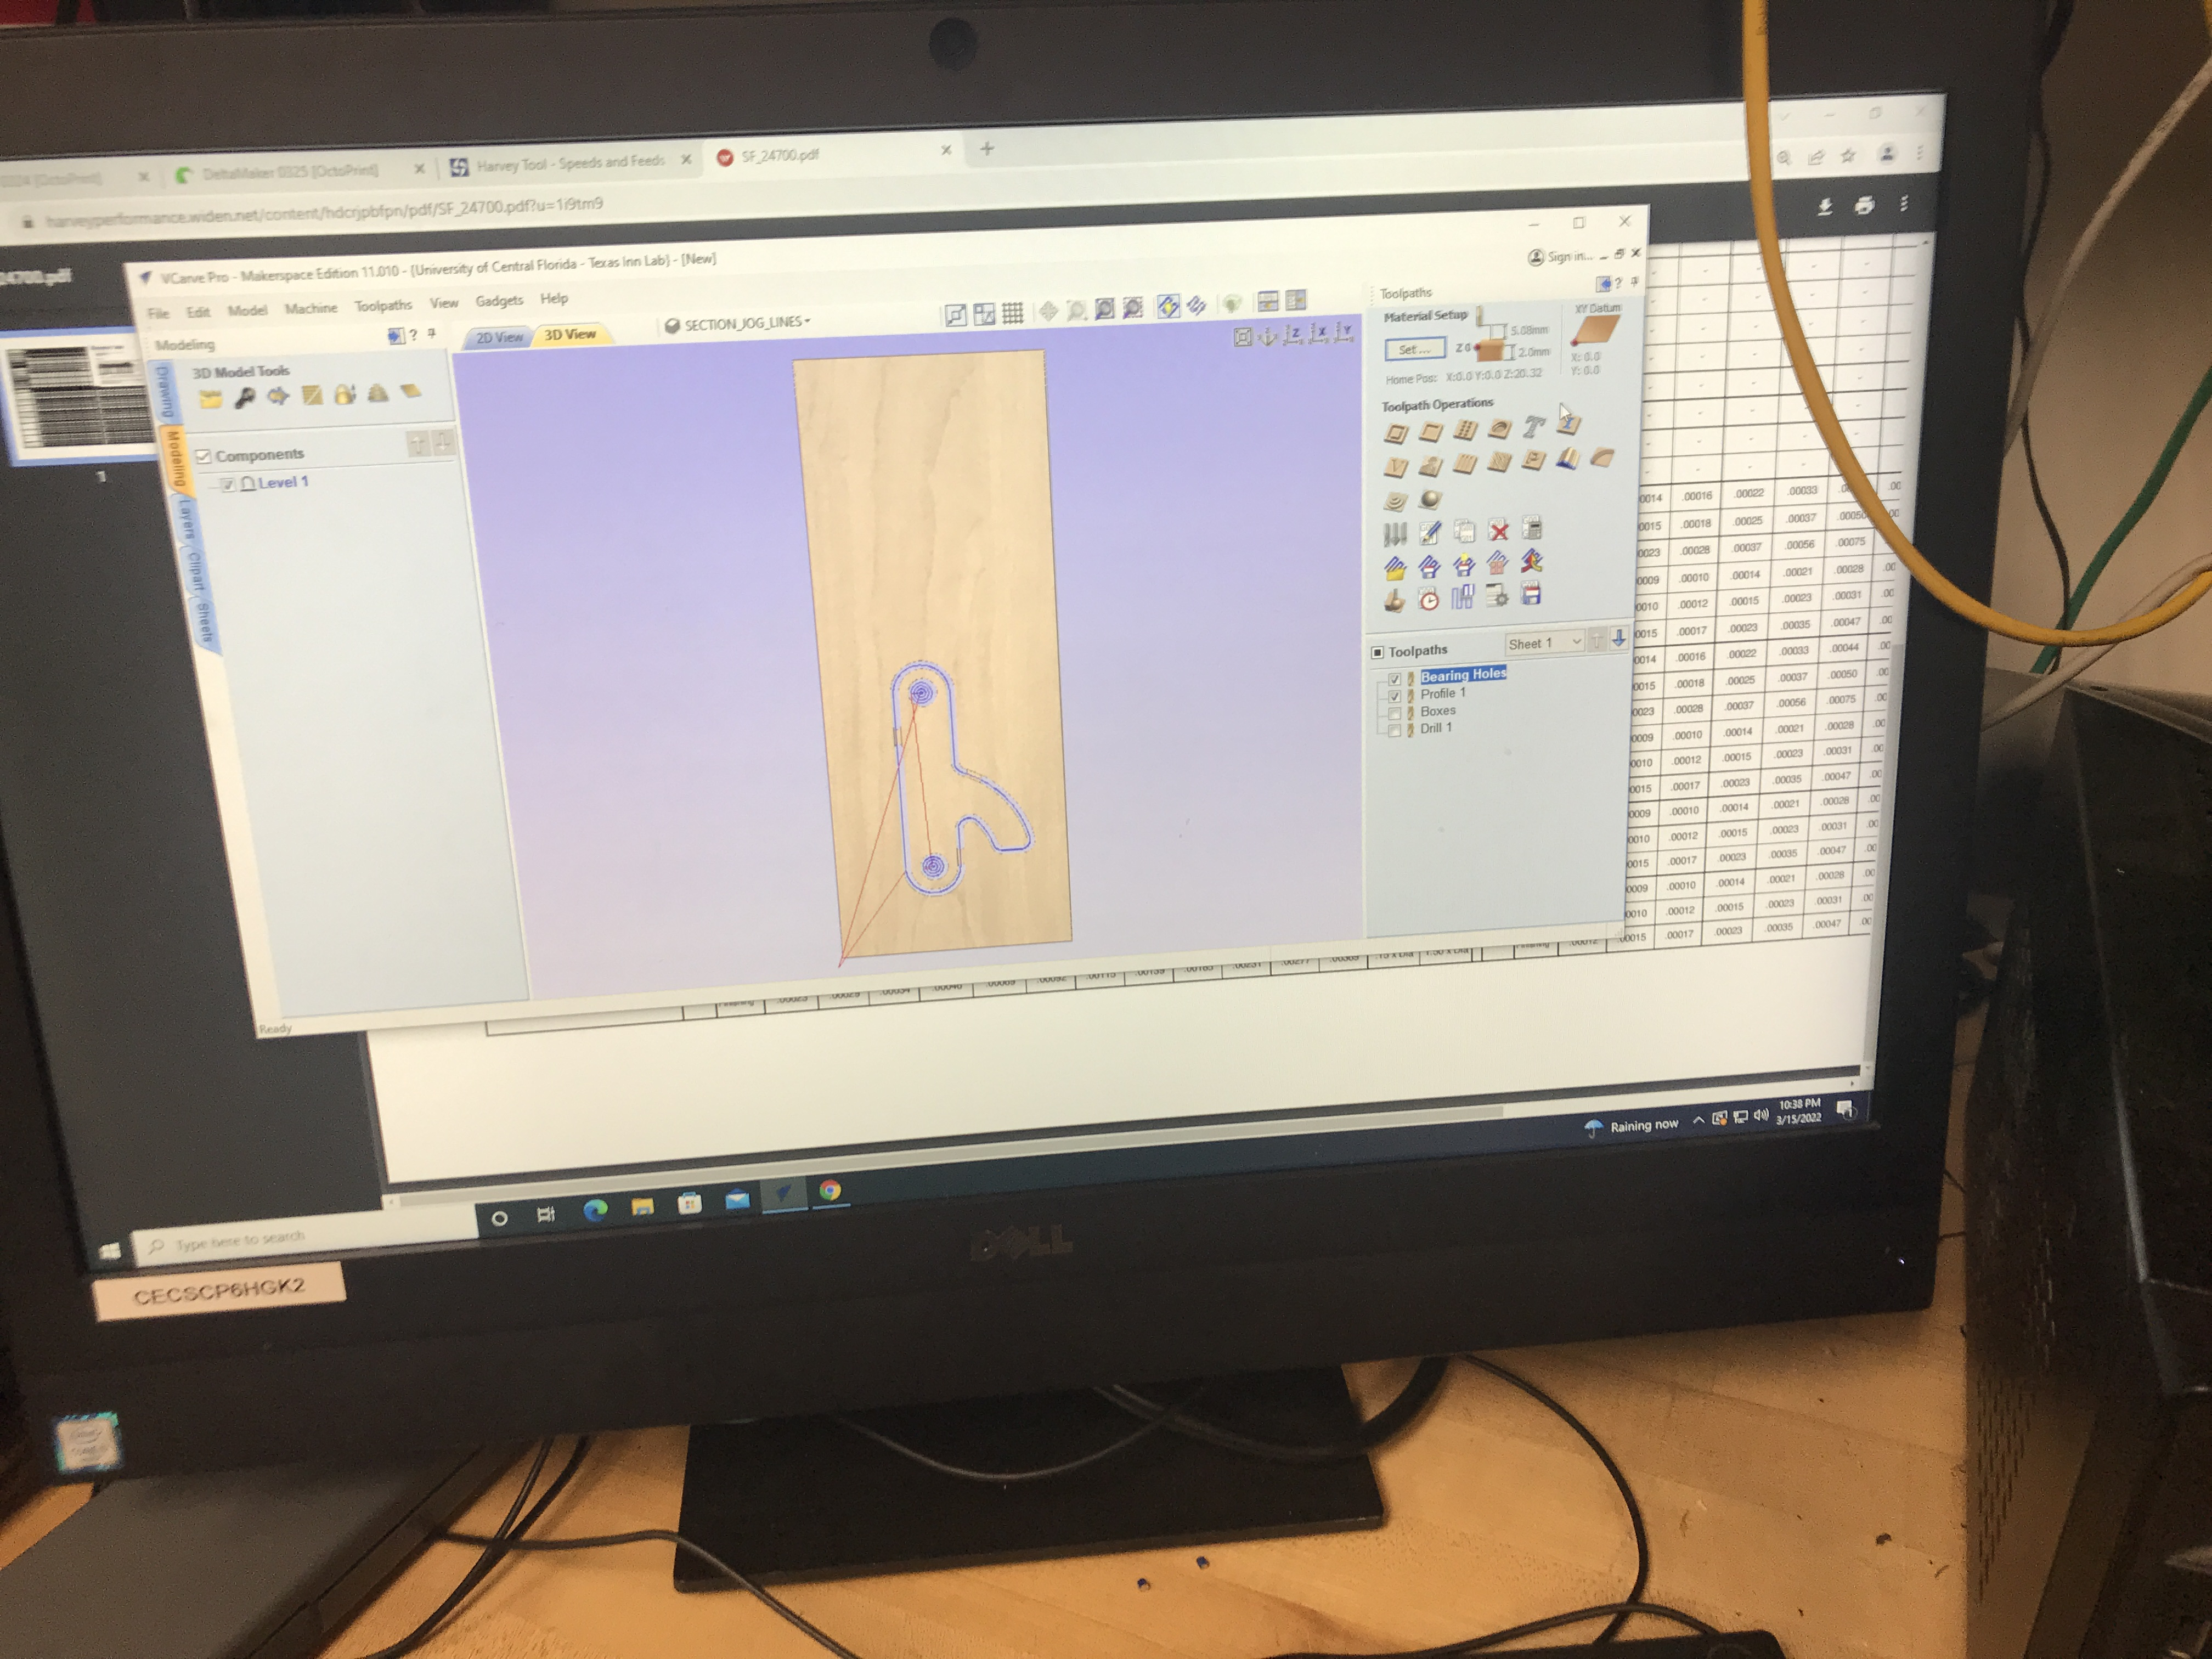
\includegraphics[width=0.95\textwidth, angle=0]{Meetings/March/03-14-22/03-14-22 2.JPG}
\caption{The software we used to prepare the file.}
\label{fig:031022_2}
\end{figure}

\begin{figure}[htp]
\centering
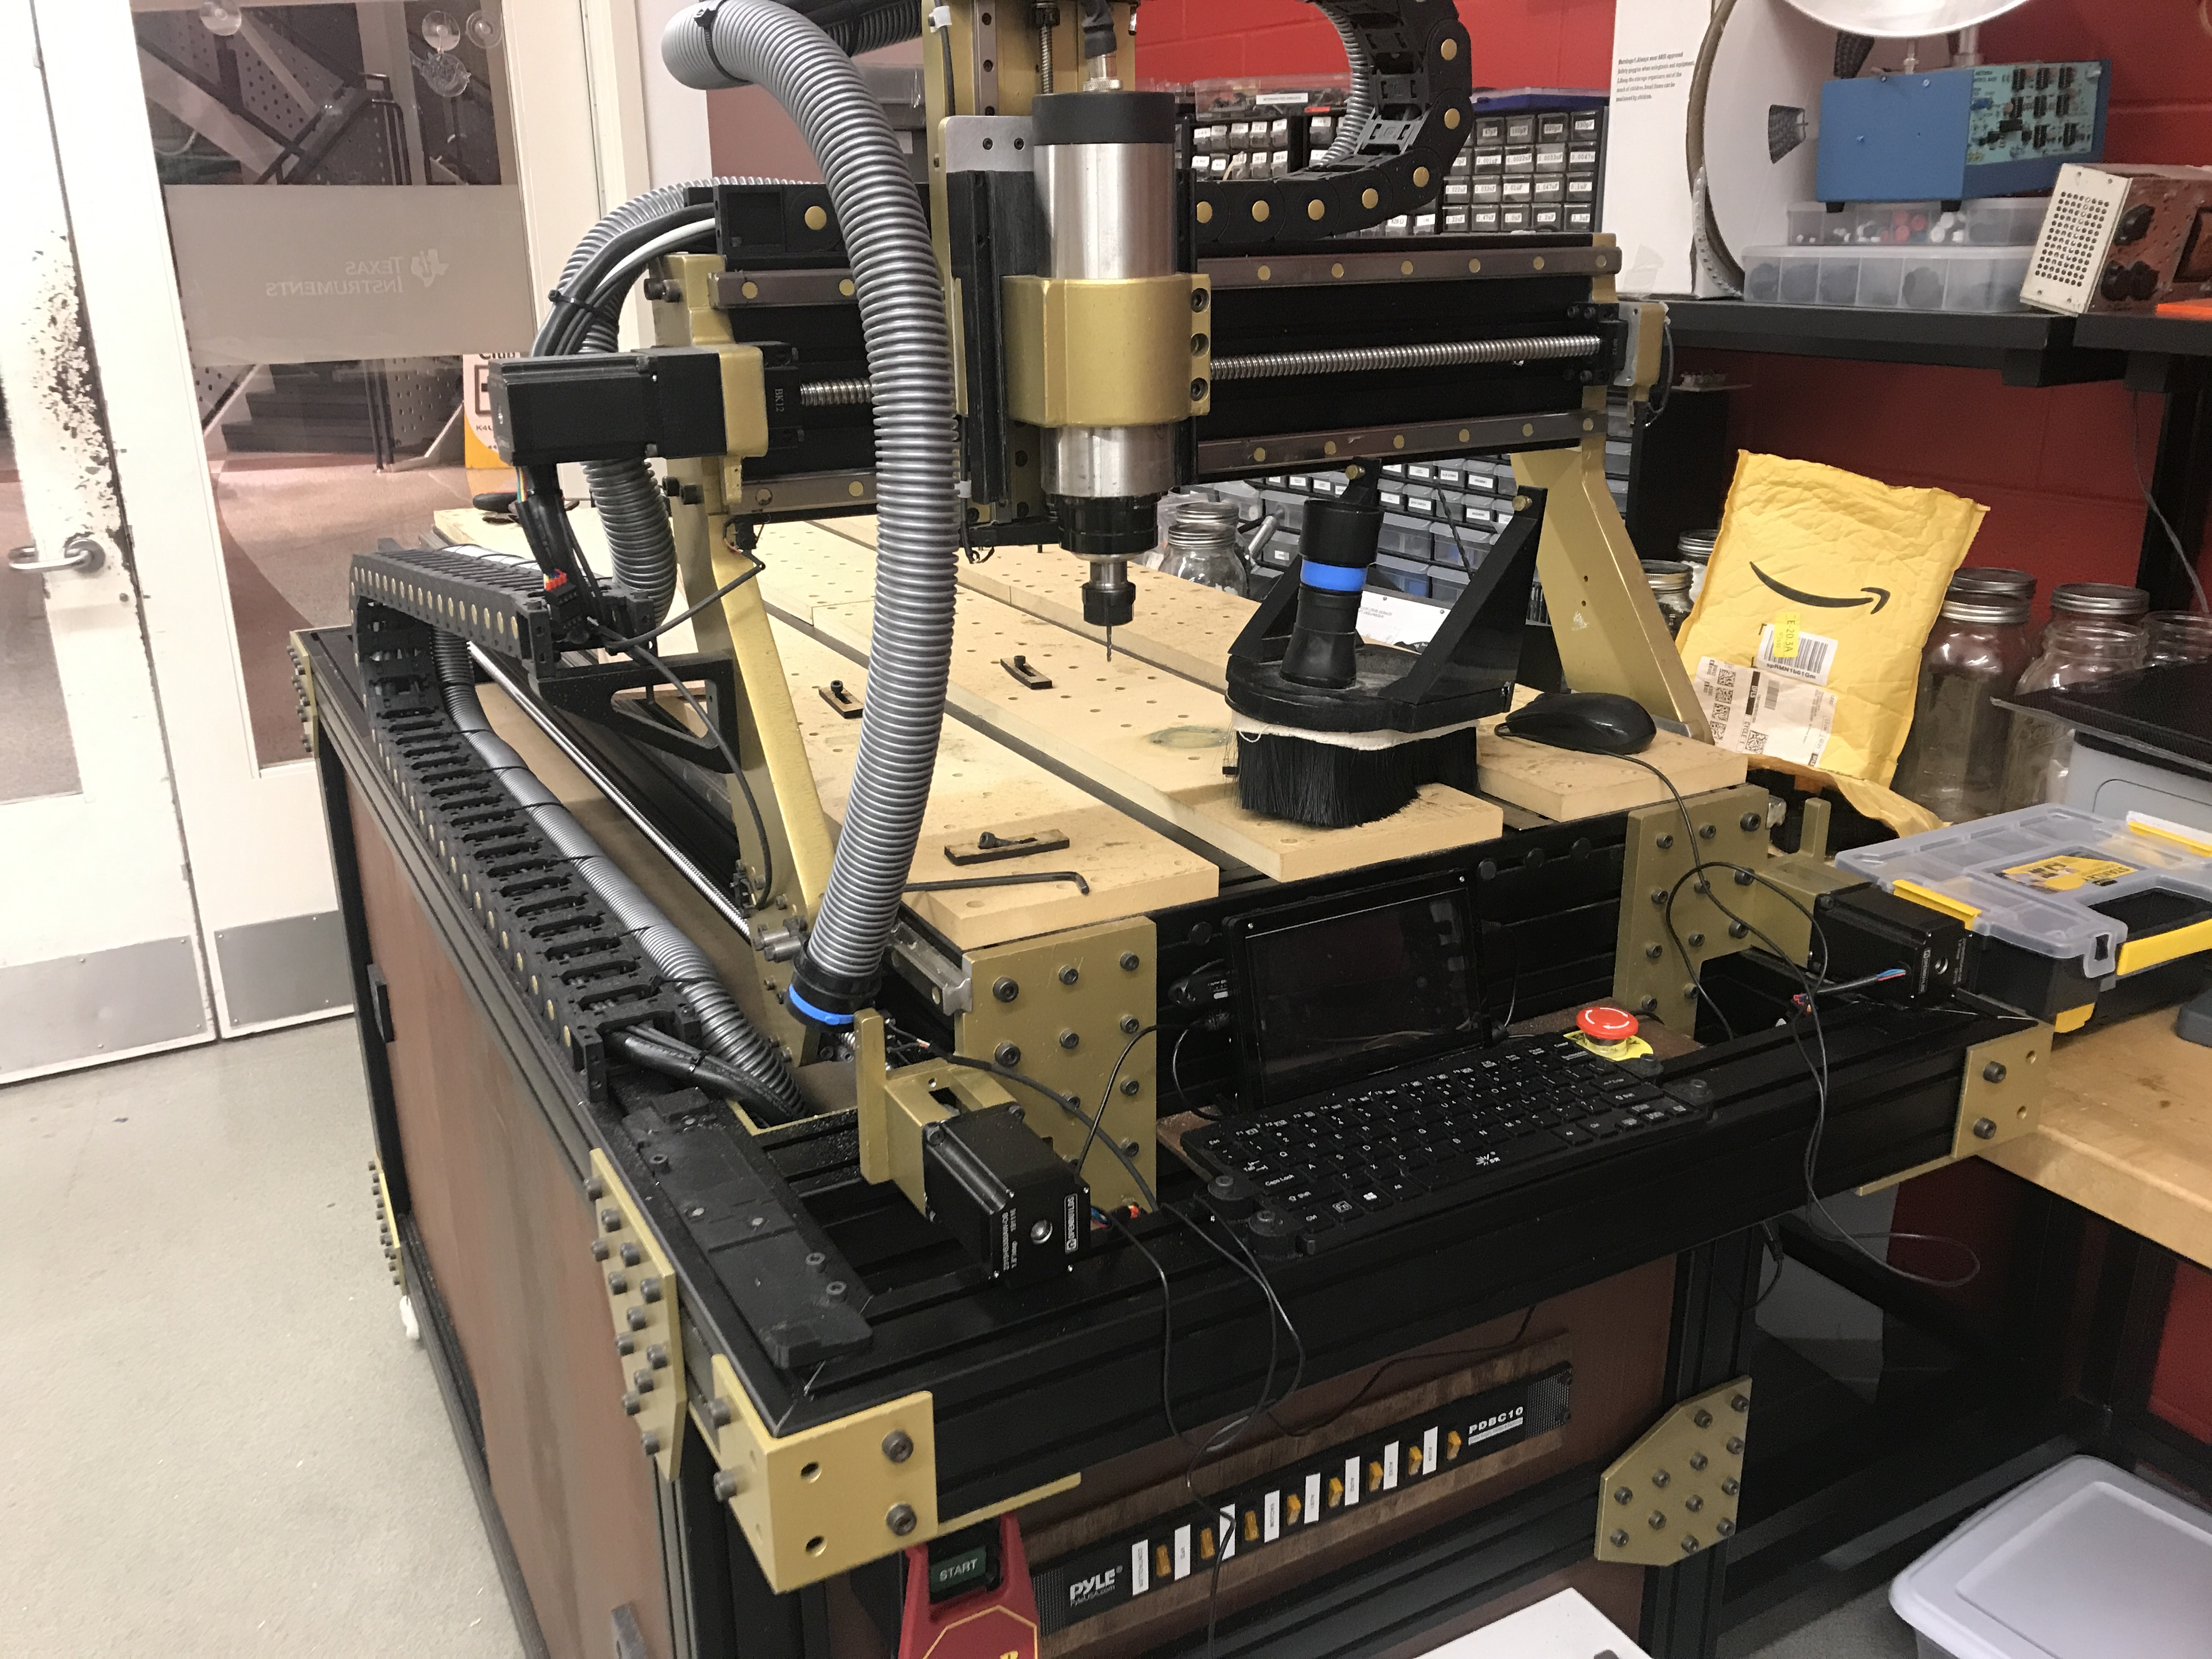
\includegraphics[width=0.95\textwidth, angle=0]{Meetings/March/03-14-22/03-14-22 3.JPG}
\caption{The CNC machine we used.}
\label{fig:031022_3}
\end{figure}

\begin{figure}[htp]
\centering
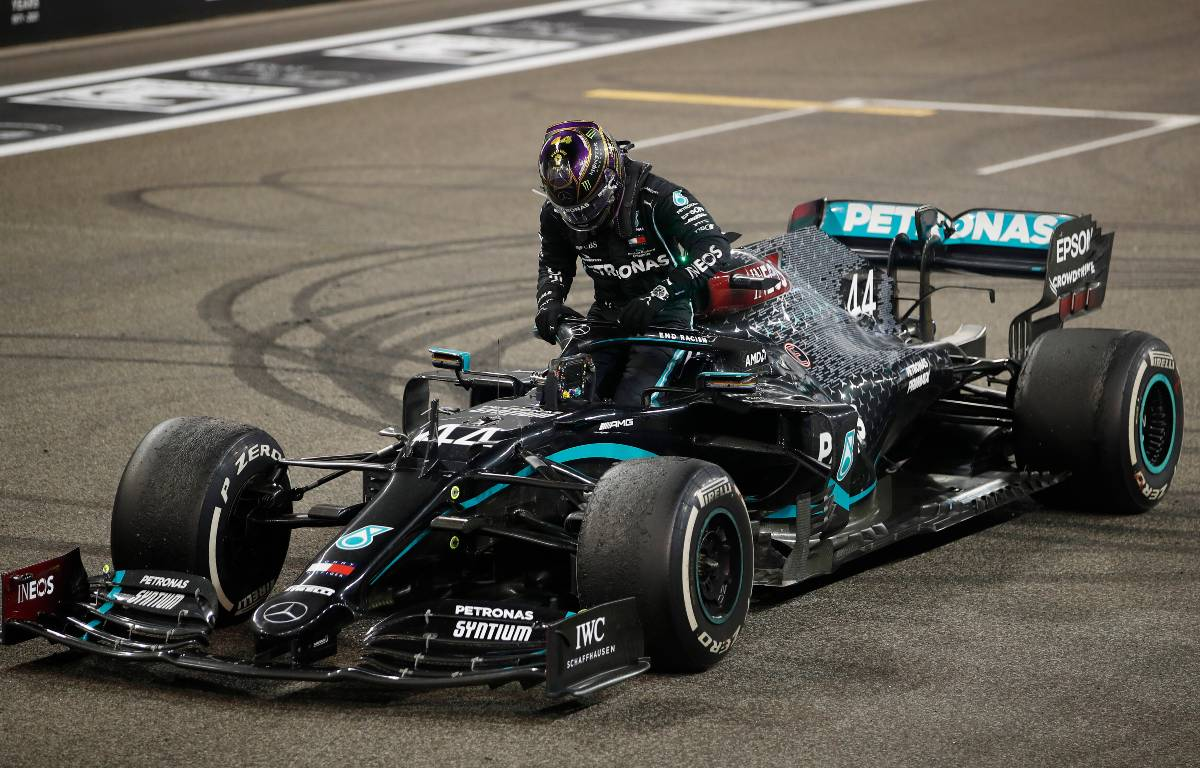
\includegraphics[width=0.95\textwidth, angle=0]{Meetings/March/03-14-22/03-14-22 4.jpg}
\caption{Lewis Hamilton's car also uses carbon fiber.}
\label{fig:031022_4}
\end{figure}






\whatsnext{
\begin{itemize}
    \item Cut out the intake plates using the fixed CNC machine.
\end{itemize} 
}

